% !TeX spellcheck = it_IT
\newpage
\section{Machine learning}
\subsection{Introduzione}
L'\textbf{apprendimento} è un principio universale per esseri viventi, per la società ma anche per le macchine. È permette di fornire l'\textbf{intelligenza} a sistemi. È un campo complesso ed in continua crescita per creare:
\begin{itemize}
	\item Computer che possano \textbf{imparare}
	\item Nuovi \textbf{strumenti} potenti ed adattivi con basi rigorose nell'informatica
\end{itemize}
Permettere alle macchine di imparare ci serve perché la quantità di dati sta aumentando esponenzialmente ed è molto difficile istruire una macchina solamente tramite istruzioni imperative.\\
Tra gli obiettivi ci sono:
\begin{itemize}
	\item Costruire \textbf{sistemi adattivi intelligenti} (e.g. robot, motori di ricerca)
	\item Creare \textbf{strumenti statistici} per analizzare i dati (data science)
	\item Affrontare \textbf{nuovi problemi} fin'ora troppo complessi (e.g. ambito medico)
\end{itemize}
\begin{example}[Email spam classification]
	\label{example:email_spam}
	Identificare tramite istruzioni rigorose quali mail sono o non sono spam è molto difficile, considerando anche che può variare da persona a persona. Il machine learning in questo caso permette di costruire una \textit{classificazione} basata su degli \textit{esempi} che si possa \textit{adattare} ai vari casi.
\end{example}
\begin{example}[Face recognition]
	Nel 2014 è stata sviluppata una rete neurale che permetteva, partendo dall'apprendimento di circa 4 milioni di immagini, di riconoscere le facce umane già viste, con una percentuale di successo del $97.25\%$ (quella umana è del $97.53$).
\end{example}
\begin{example}[Go]
	Il gioco del Go, in quanto molto complesso (anche più degli scacchi), si è adattato molto bene al machine learning, che con il tempo è riuscito a battere gli umani e a diventare sempre più esperto.
\end{example}
\begin{example}[Traduzione]
	Un'altra applicazione molto famosa sono i sistemi di traduzione automatica, come Google Translate dal 2016 o DeepL dal 2017.
\end{example}
\begin{example}[Medicina]
	Il machine learning in ambito medico può aiutare in diversi aspetti: dalla diagnosi alla terapia, alle medicine personalizzate, al monitoraggio della salute e persino alla progettazione delle medicine stesse.\\
	Uno degli esempi più famosi è quello della rete neurale che permette di riconoscere il cancro alla pelle con l'accuratezza di un dermatologo certificato.
\end{example}
\begin{example}[Musica]
	Anche nell'arte, in particolare della musica, ci sono diversi esempi di Machine Learning, come AIVA, una rete neurale che è partita dalla composizione di un brano per pianoforte ed è arrivata ad orchestre e colonne sonore per videogiochi.
\end{example}
\begin{note}[Premio Turing]
	Il premio Turing del 2018 è stato vinto da tre professori, il Dr. Hinton, il Dr. LeCun e il dottor Bengio, per il loro lavoro innovativo che ha reso le reti neurali profonde un componente fondamentale per l'informatica moderna.
\end{note}

\subsubsection{Quando?}
Il machine learning deve essere utilizzato quando può essere \textbf{utile} (\textbf{opportunity}):
\begin{itemize}
	\item Per problemi di cui c'è poca o nessuna teoria
	\item In presenza di dati incerti, distorti o non completi
	\item In ambienti dinamici che non possono essere previsti in anticipo
\end{itemize}
e con criterio in base a ciò di cui ha bisogno (\textbf{awareness}):
\begin{itemize}
	\item Una fonte di apprendimento
	\item Si deve accettare che i risultati avranno una certa tolleranza
\end{itemize}

\begin{note}
	Il machine learning non è una metodologia approssimata ma bensì un metodo rigoroso per trovare una funzione approssimata che gestisca il problema complesso. Viene quindi definito \textbf{soft computing}, ovvero aperto a nuove possibilità (e.g. la biologia).
\end{note}

\subsection{Sistema predittivo}
Un sistema si compone dai \textbf{dati}, ovvero le osservazioni del mondo reale, da un \textbf{modello}, che può migliorare tramite apprendimento ed è quindi composto anche da \textit{task}, \textit{algoritmo di apprendimento} e metodo di \textit{validazione}, e da una \textbf{previsione}. 
\begin{center}
	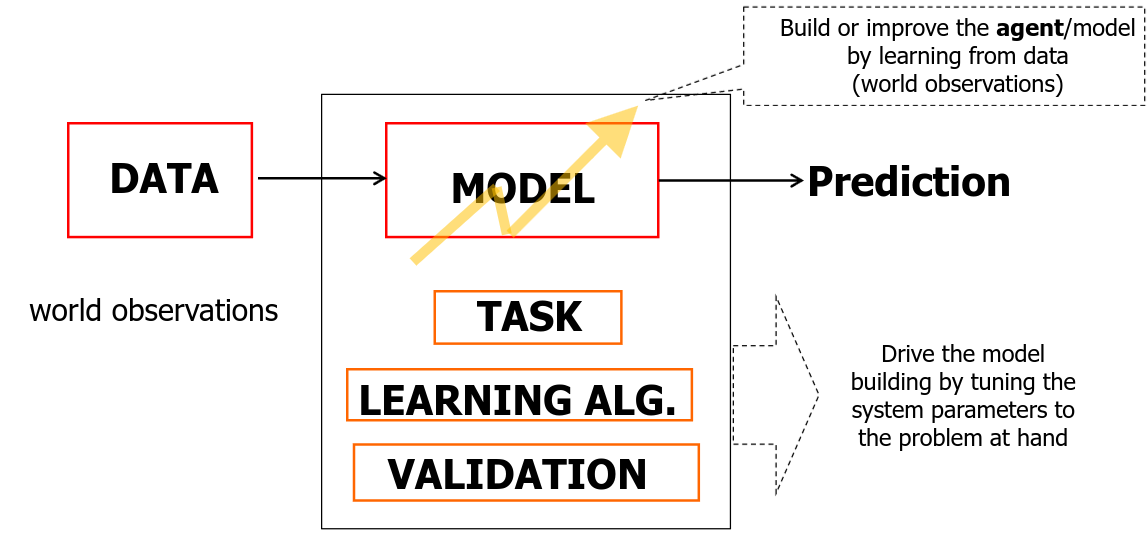
\includegraphics[scale=0.4]{predictive_system.png}
\end{center}

Il machine learning consiste nel ricostruire una \textbf{funzione} a partire dai dati.
\begin{example}[Riconoscimento della scrittura]
	Partiamo dai dati in \textbf{ingresso}: una raccolta di immagini di scrittura a mano di cifre sotto forma di array e matrici. Vogliamo costruire un modello che, ricevuta in input un'immagine di scrittura a mano, ne predica le cifre.
	
	\begin{center}
		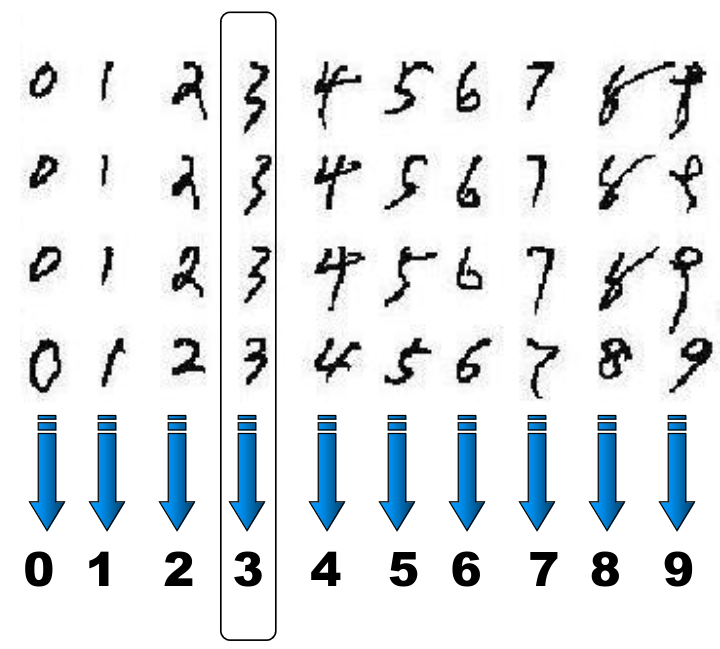
\includegraphics[scale=0.2]{hand_writing_recognition.png}
	\end{center}
	Il problema ha quindi una soluzione difficile da formalizzare (presenza di rumore e ambiguità nei dati) ma è facile ottenere dei dati da cui far apprendere il modello.\\
\end{example}

L'apprendimento può essere di due tipi:
\begin{itemize}
	\item \textbf{Supervisionato}: a partire da una serie di dati \textbf{supervisionati} (sappiamo che etichetta hanno), si crea una funzione che si possa applicare ad altri casi
	\item \textbf{Non supervisionato}: a partire da una serie di dati non etichettati cerchiamo \textbf{raggruppamenti naturali} come:
	\begin{itemize}
		\item Clustering
		\item Modellazione della densità dei dati
		\item Preprocessing, visualizzazione, riduzione dimensionale
	\end{itemize}
\end{itemize}

\subsubsection{Apprendimento supervisionato}
\begin{definition}[Task]
	Dato un insieme di \textbf{esempi} etichettati del tipo
	\begin{equation*}
		<input,output>=(\textbf{x},d)
	\end{equation*}
	per una \textbf{funzione} sconosciuta $f$, di cui conosciamo il valore solo per i punti in ingresso (\textbf{target value} $d$).\\
	Dobbiamo trovare una buona \textit{approssimazione} a $f$, ovvero un \textbf{ipotesi} $h$ che può essere usata per fare previsioni su dati mai visti $x'$.\\
	Il \textbf{target} può essere:
	\begin{itemize}
		\item \textbf{Categorico} per i problemi di \textbf{classificazione}: $f(\textbf{x})$ restituisce la presunta corretta classe tra $\{1,2,\ldots, k\}$
		\item \textbf{Numerico} per i problemi di \textbf{regressione}, dove $f(\textbf{x})$ restituisce valori continui
	\end{itemize}
\end{definition}

\begin{example}
	Alcuni esempi di funzioni:
	\begin{itemize}
		\item Riconoscimento di scrittura
		\begin{itemize}
			\item $\textbf{x}$: dati dalle immagini dei caratteri
			\item $f(\textbf{x})$: lettere dell'alfabeto
		\end{itemize}
		\item Diagnosi di malattie da cartella clinica
		\begin{itemize}
			\item $\textbf{x}$: dati sul paziente (sintomi, analisi di laboratorio)
			\item $f(\textbf{x})$: malattia o terapia consigliata
			\item Training set: cartella clinica del paziente
		\end{itemize}
		\item Riconoscimento facciale
		\begin{itemize}
			\item $\textbf{x}$: immagine della faccia della persona
			\item $f(\textbf{x})$: nome della persona
		\end{itemize}
		\item Riconoscimento dello spam
		\begin{itemize}
			\item $\textbf{x}$: email
			\item $f(\textbf{x})$: spam o non spam
		\end{itemize}
	\end{itemize}
\end{example}

\begin{definition}[Modello]
	Un modello ha come obiettivo quello di descrivere le relazioni tra i dati sulla base di un task. Definisce la classe della funzione che la macchina può implementare, ovvero lo \textbf{spazio delle ipotesi} (e.g. $h(\textbf{x}, \textbf{w})$ dove $w$ sono parametri astratti).
\end{definition}
\begin{definition}[Esempi di training]
	Un esempio della forma
	\begin{equation*}
		(\textbf{x}, f(\textbf{x})+noise)
	\end{equation*}
	dove $\textbf{x}$ è di solito un vettore di caratteristiche e $d=f(\textbf{x})+noise$ è il \textbf{target value}.
\end{definition}
\begin{definition}[Funzione obiettivo]
	La vera funzione $f$.
\end{definition}
\begin{definition}[Ipotesi]
	Una proposta di funzione $h$ che si crede essere simile a $f$. Un'espressione in un determinato \textbf{linguaggio} (e.g. logico, numerico o probabilistico) che descrive la relazione tra i dati.
\end{definition}
\begin{definition}[Spazio delle ipotesi]
	L'insieme di tutte le ipotesi che possono in teoria essere date in output dall'algoritmo.
\end{definition}

\noindent Alcuni modelli sono:
\begin{itemize}
	\item Modelli \textbf{lineari}, dove ogni rappresentazione di $h$ definisce uno spazio continuo di ipotesi. Ogni assegnamento di \textbf{$w$} è un'ipotesi differente. Ad esempio
	\begin{equation*}
		h_w(x)=w_1x+w_0 \quad h_w(x) = 0.232x + 246
	\end{equation*}
	\item \textbf{Regole simboliche}: lo spazio delle ipotesi è composto da rappresentazioni discrete. Si possono applicare diverse regole, ad esempio:
	\begin{lstlisting}[language=Python]
		if (x_1=0) and (x_2=1) then h(x)=1
		else h(x)=0
	\end{lstlisting}
	\item Modelli \textbf{probabilistici}: si fa una stima di $p(\textbf{x},y)$
	\item Modelli basati su \textbf{istanze}: predicono il valore medio $y$ dei vicini più prossimi (memory based)
\end{itemize}

\begin{definition}[Algoritmo di apprendimento]
	È un algoritmo che si basa sui dati, sulle task e sul modello ed impara con una ricerca euristica attraverso le ipotesi nello spazio $H$ delle migliori ipotesi (di solito cercando $h$ con l'errore minimo che si approssimi meglio alla funzione obiettivo).
	\begin{center}
		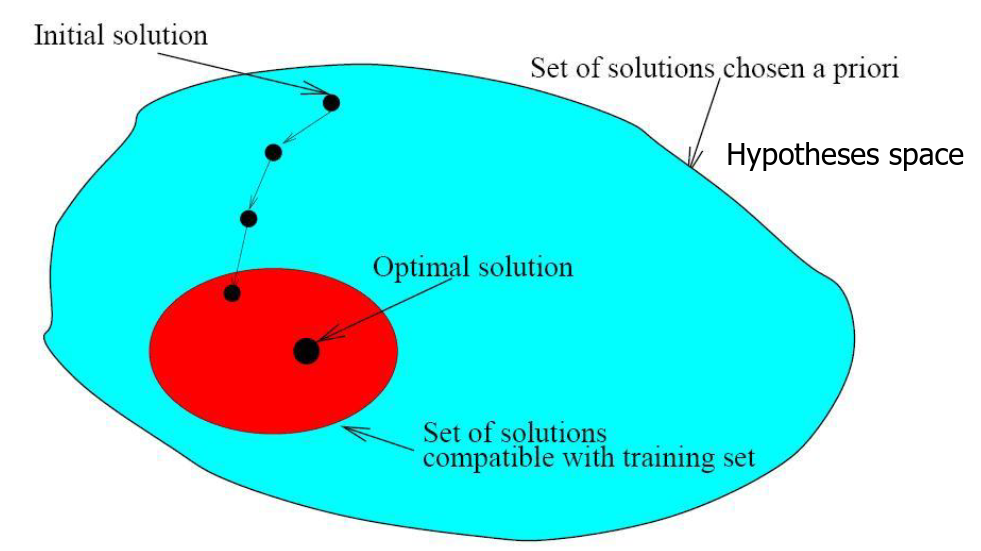
\includegraphics[scale=0.2]{learning_alg_search.png}
	\end{center}
\end{definition}

\begin{note}
	L'insieme $H$ potrebbe non coincidere con tutte le possibili funzioni e la ricerca quindi non può essere esaustiva: deve fare determinate assunzioni.
\end{note}

\begin{definition}[Funzione buona]
	Definiamo una funzione trovata come buona se è \textbf{generale}, ovvero in base a quanto è accurata nel predire i valori per nuovi dati. Ci sono quindi due fasi:
	\begin{itemize}
		\item \textbf{Learning}: il modello viene costruito da dati noti
		\item \textbf{Test}: il modello viene applicato a nuovi esempi e vengono valutate le capacità predittive in maniera \textbf{generale}
	\end{itemize}
\end{definition}
\begin{note}[Performance]
	Nel Machine Learning la performance indica l'accuratezza del modello nel predire un risultato, stimata dall'errore computo nella fase di test.
\end{note}

\subsection{Concept learning}
Il concept learning si tratta di inferire una \textbf{funzione booleana} a partire da esempi positivi o negativi.
\begin{definition}[Esempio]
	Definiamo come esempio la seguente coppia:
	\begin{equation*}
		<x,c(x)> \in D
	\end{equation*}
\end{definition}
\begin{definition}[Soddisfa]
	Una funzione $h:X\to\{0,1\}$ soddisfa $x$ se
	\begin{equation*}
		h(x)=1
	\end{equation*}
\end{definition}
\begin{definition}[Consistenza]
	Un'ipotesi $h$ è consistente con:
	\begin{itemize}
		\item un \textbf{esempio} $<x,c(x)> \quad x \in X$ se $h(x) = c(x)$
		\item un \textbf{insieme di esempi} $D$ se $\forall <x,c(x)> \in D \Longrightarrow h(x) = c(x)$
	\end{itemize}
\end{definition}
\begin{definition}[Problema mal posto]
	Un problema si dice mal posto quando viola:
	\begin{itemize}
		\item L'\textbf{esistenza}
		\item L'\textbf{unicità}
		\item La \textbf{stabilità}
	\end{itemize}
	della soluzione.
\end{definition}
\begin{definition}[Spazio delle ipotesi]
	Dati $n$ input binari, lo spazio delle ipotesi è:
	\begin{equation}
		\lvert H \rvert = 2^{\#-instances}=2^{2^n}
	\end{equation}
\end{definition}
\begin{example}[Funzioni booleane]
	Dati dei valori booleani in input di cui sappiamo l'output, dobbiamo determinare la funzione booleana.
	\begin{table}[!h]
		\centering
		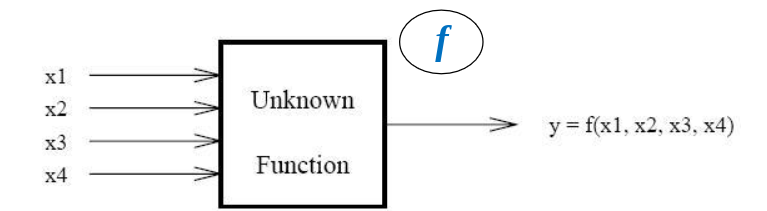
\includegraphics[scale=0.3]{boolean_function.png}
		\begin{tabular}{cccc|c}
			$x_1$ & $x_2$ & $x_3$ & $x_4$ & y \\
			\hline
			0 & 0 & 1 & 0 & 0 \\
			0 & 1 & 0 & 0 & 0 \\
			0 & 0 & 1 & 1 & 1 \\
			1 & 0 & 0  &1 & 1 \\
			0 & 1 & 1 & 0 & 0 \\
			1 & 1 & 0 & 0 & 0 \\
			0 & 1 & 0 & 1 & 0 \\
			\hline
		\end{tabular}
	\end{table}
	\\Questo è una problema \textbf{mal posto} in quanto ci sono più funzioni che potrebbero dare questo risultato (\textbf{unicità}).
	Dati quattro input binari, abbiamo $2^{2^4}= 65536 $ possibili funzioni che dobbiamo esplorare interamente per trovare quella corretta.\\
	È necessario lavorare con uno spazio ristretto di ipotesi $H$.
\end{example}
\begin{definition}[Lookup table]
	Un possibile modello di ML è quello di \textit{Lookup Table}, dove l'algoritmo sa a memoria le risposte che gli sono state date in ingresso e sa rispondere solo se gli viene chiesta una di quelle.
\end{definition}
\subsubsection{Conjective Rules}
Tramite il costrutto \textbf{AND} possiamo ridurre lo spazio delle ipotesi. Considerando dei letterali $l_i$ come pezzo di una stringa di lunghezza $n$, abbiamo:
\begin{itemize}
	\item Letterali \textbf{positivi} (e.g. $h_1=l_2$, $h2=l_1 \land l_2$, $h_3=true$): $\lvert H \rvert = 2^n$
	\item Letterali anche \textbf{negativi} (e.g. $not(l_i)$): $\lvert H \rvert = 3^n + 1$
\end{itemize}

\begin{example}[Enjoy sport]
	\label{example:enjoy_sport}
	Supponiamo di avere determinati \textbf{attributi} relativi al tempo meteorologico e in corrispondenza se una persona vuole o meno fare sport.\\
	Abbiamo quindi $X$ \textbf{istanze}, una \textbf{funzione obiettivo} ($c:EnjoySport \: X \to \{0,1\}$) e un \textbf{training set} $l$ composto da coppie di tipo $<x_n,c(x_l)$
	\begin{table}[!h]
		\centering
		\begin{tabular}{|ccccccc|}
			\hline
			Sky & Temp & Humid & Wind & Water & Forecast & Enjoy \\
			\hline
			Sunny & Warm & Normal & Strong & Warm & Same & Yes \\
			Sunny & Warm & High & Strong & Warm & Same & Yes \\
			Rainy & Cold & High & Strong & Warm & Change & No \\
			Sunny & Warm & High & Strong & Cool & Change & Yes \\
			\hline
		\end{tabular}
	\end{table}
	\\Rappresentiamo ogni \textbf{ipotesi} come insieme di vincoli sugli attributi scelto tra:
	\begin{itemize}
		\item Un valore specifico, e.g. $Water=Warm$
		\item Un valore che non ci interessa, e.g. $Water=?$
		\item Nessun valore permesso (ipotesi nulla), e.g. $Water=\emptyset$
	\end{itemize}
	Una possibile \textit{ipotesi} (per cui quindi una persona va a fare sport) è la seguente:
	\begin{equation*}
		Sky=Sunny \land Wind=Strong \land Forecast=Same
	\end{equation*}
	L'ipotesi più specifica avrà tutti valori \textit{nulli} mentre quella più generale avrà tutti valori che non ci interessano.\\
	L'\textbf{obiettivo} è quello di trovare un'ipotesi $h$ tale che $h(x)=c(x) \forall x \in X$.
	\begin{note}
		Per ora assumiamo che ogni ipotesi che approssimi la funzione obiettivo correttamente sui training examples, approssimerà anche la funzione sugli esempi non osservati. In generale uno dei problemi fondamentali del ML è la differenza tra analisi teorica ed empirica.
	\end{note}
	Per questo esempio abbiamo
	\begin{equation*}
		3 \cdot 2 \cdot 2 \cdot 2 \cdot 2 \cdot 2 = 96
	\end{equation*}
	istanze distinte e $2^{96}$ \textbf{funzioni possibili}. Possiamo semplificare prendendo le ipotesi \textit{sintatticamente} distinte, ovvero $5\cdot 4 \cdot 4 \cdot4 \cdot 4 \cdot 4 = 5120$, oppure quelle \textit{semanticamente} distinte, ovvero $1+4\cdot3\cdot3\cdot3\cdot3\cdot3 = 973$.
\end{example}

\begin{definition}[Più generale]
	Siano $h_j$ e $h_k$ funzioni booleane definite su $X$. $h_j$ è più generale o uguale di $h_k$ se e solo se:
	\begin{equation}
		\forall x \in X : [(h_k(x) = 1) \to (h_j(x)=1)]
	\end{equation}
\end{definition}
In questo modo possiamo imporre un ordinamento sulle \textit{ipotesi}, del tipo $l_i : l_1 \geq (l_1 \land l_2)$, e strutturarne lo spazio dalle più specifiche alle più generali.
\begin{center}
	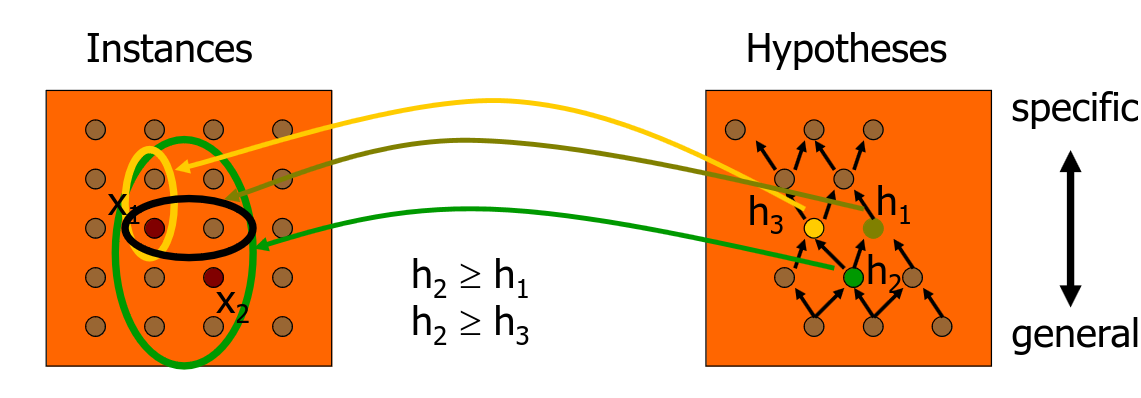
\includegraphics[scale=0.3]{hyp_ordin.png}
\end{center}
\subsubsection{Find-S}
Un algoritmo per cercare una soluzione prevede di ordinare le ipotesi e cercare la più specifica senza bisogno di enumerarle tutte:
\begin{enumerate}
	\item Inizializza $h$ all'ipotesi più specifica in $H$
	\item Per ogni training istance $x$ \textbf{positiva}:
	\begin{lstlisting}
		for each attribute a[i] in h
			if a[i] in h is statisfied by x
				do nothing
			else
				replace a[i] in h by the next more general costraint satisfied by x
	\end{lstlisting}
	\item Restituisci l'ipotesi $h$
\end{enumerate}
\begin{example}
	Partendo dall'esempio \ref{example:enjoy_sport}, facciamo i seguenti passi:
	\begin{enumerate}
		\item $h_0=<\emptyset,\emptyset,\emptyset,\emptyset,\emptyset>$ è la prima ipotesi
		\item Non soddisfa $x_1$. Mettiamo tutti gli attributi in modo che soddisfino al minimo $x_1$. Otteniamo $h_1=<Sunny,Warm,Normal,Strong,Warm,Same>$
		\item $h_1$ non soddisfa $x_2$. Per soddisfarla generalizziamo ulteriormente l'attributo $Humid$, ottenendo $h_2=<Sunny,Warm,?,Strong,Warm,Same>$
		\item $x_3$ è negativa, quindi non la consideriamo
		\item $h_2$ non soddisfa $x_4$. Generalizziamo gli attributi $Water$ e $Forecast$ e otteniamo \\$h_3=<Sunny,Warm,?,Strong,?,?>$
	\end{enumerate}
\end{example}
Questo algoritmo permette di trovare l'ipotesi più specifica che sia consistente con il training example (anche per gli esempi negativi).\\
Un problema è che non c'è \textbf{tolleranza al rumore}, ovvero che non valutando gli esempi negativi non sappiamo se ci sono delle contraddizioni. Inoltre trova solo una soluzione.

\subsubsection{List-Then-Eliminate}
L'idea è di ottenere una descrizione dell'insieme di tutte le ipotesi che siano consistenti con il training example.
\begin{definition}[Version space]
	Il version space $VS_{H,D}$ rispetto allo spazio delle ipotesi $H$ e al training set $D$ è il sottoinsieme delle ipotesi che sono consistenti con tutti i casi del training examples
	\begin{equation}
		VS_{H,D}=\{h \in H \vert Consistent(h,D)\}
	\end{equation}
\end{definition}
L'algoritmo prevede i seguenti passi:
\begin{enumerate}
	\item Faccio una lista di tutte le ipotesi (VersionSpace) $H$
	\item Per ogni training example $<x,c(x)$ rimuovo ogni ipotesi del VS che è inconsistente con quell'esempio
	\item Restituisco il VS
\end{enumerate}
È un algoritmo irrealistico in quanto dovremmo enumerare tutte le ipotesi.
\subsubsection{Candidate Elimination}
Per evitare di enumerare tutte le ipotesi, possiamo definire il Version Space con dei limiti generali e specifici.
\begin{definition}[General boundary]
	Il limite generale $G$ di un version space $VS_{H,D}$ è l'insieme delle ipotesi più generali in $H$ consistenti con $D$.
\end{definition}
\begin{definition}[Specific boundary]
	Il limite specifico $G$ di un version space $VS_{H,D}$ è l'insieme delle ipotesi più specifiche in $H$ consistenti con $D$.
\end{definition}
\begin{theorem}
	Ogni membro del version space si trova tra il \textbf{general} e lo \textbf{specific} boundary.
	\begin{equation}
		VS_{H,D} = \{h \in H \vert (\exists s \in S) (\exists g \in G) (g\geq h \geq s)\}
	\end{equation}
\end{theorem}
L'algoritmo prevede, per ogni training example $d$, dato $G$ l'insieme delle ipotesi più generali e $S$ quello delle ipotesi più specifiche:
\begin{itemize}
	\item Se $d$ è \textbf{positivo}:
	\begin{enumerate}
		\item Rimuovo da $G$ ogni ipotesi che non sia consistente con $d$
		\item Per ogni ipotesi $s$ che non è consistente con $d$:
		\begin{itemize}
			\item Rimuovo $s$ da $S$
			\item Aggiungo a $S$ tuute le ipotesi $h$ sufficientemente generalizzate in modo che $h$ sia consistente con $d$ e che alcuni elementi di $G$ siano più generali di $h$
			\item Rimuovo da $S$ ogni ipotesi che sia più generale di un'altra ipotesi in $S$
		\end{itemize}
	\end{enumerate}
	\item Se $d$ è \textbf{negativo}:
	\begin{enumerate}
		\item Rimuovo da $S$ ogni ipotesi che non sia consistente con $d$
		\item Per ogni ipotesi $g$ che non è consistente con $d$:
		\begin{itemize}
			\item Rimuovo $g$ da $G$
			\item Aggiungo a $G$ tuute le ipotesi $h$ sufficientemente specializzate in modo che $h$ sia consistente con $d$ e che alcuni elementi di $S$ siano più specializzati di $h$
			\item Rimuovo da $G$ ogni ipotesi che sia meno generale di un'altra ipotesi in $G$
		\end{itemize}
	\end{enumerate}
\end{itemize}
Per \textbf{classificare} i nuovi dati, testiamo la loro consistenza con il version space e vediamo con quante delle ipotesi dà risultato positivo o negativo.

\subsubsection{Bias induttivo}
Il version space non può rappresentare le disgiunzioni (e.g. soleggiato O nuvoloso). Per rimuovere il bias possiamo scegliere uno spazio delle ipotesi $H$ che contenga ogni singolo concetto, ovvero tutti i possibili sottoinsiemi di $X$. Se abbiamo ad esempio $\lvert X \rvert=96$ allora ci sono $\lvert P(X)\rvert = 2^{96}$ concetti distinti. \\
Questa generalizzazione, oltre ad aumentare il tempo necessario per la ricerca, impedisce al modello di classificare nuovi esempi che non siano del training set.
\begin{definition}[Unbiased learner]
	Un unbiased learner non è in grado di generalizzare, in quanto ogni istanza non osservata sarà classificata positivamente da metà delle ipotesi e negativamente dall'altra metà. Ci ritroveremmo quindi con una \textbf{Lookup Table}.
\end{definition}
\noindent Le restrizioni che si fanno sono quindi \textbf{necessarie} per potere fare una generalizzazione. È importante quindi caratterizzare il bias utilizzato e capire qual'è il migliore da scegliere.

\begin{definition}[Inductive bias]
	Il bias induttivo di una algoritmo $L$ è ogni minimo insieme di assunzioni $B$ tali che per ogni concetto obiettivo $c$ e il corrispondente training data $D_c$
	\begin{equation}
		(\forall x_i \in X)[B \land D_c \land x_i] \vdash L(x_i, D_c)
	\end{equation}
	In pratica posso trasformarlo in un sistema \textbf{deduttivo}.
\end{definition}
Negli algoritmi visti fin'ora abbiamo trovato i seguenti bias:
\begin{itemize}
	\item \textbf{Lookup table}: nessun bias
	\item \textbf{Find-S}: lo spazio delle ipotesi contiene il target concept e tutte le istanza sono negative a meno che gli esempi positivi non ci dicano il contrario
	\item \textbf{Candidate Elimination}: lo spazio delle ipotesi contiene il target concept
\end{itemize}